\chapter{Introducción}
\section{Objetivos}



El principal objetivo de la tesis es obtener una implementación del método de dinámica molecular basada en GPU, que siga un modelo de interacción de Lennard-Jones (potencial de no-unión), 
y que resuelva el cálculo de las fuerzas utilizando valores tabulados en el sistema de memoria provisto por la arquitectura. 

La forma funcional que describe el potencial de Lennard-Jones permitiría obtener una buena aproximación del valor utilizando una tabla de resultados precalculados. 
Además, el sistema de memorias de la arquitectura, que ha evolucionado considerablemente desde su creación, permite recuperar de forma eficiente el valor asociado en un esquema de tablas. 
De esta forma, se espera que la modificación resulte en una mejora de la performance manteniendo la correctitud en los resultados de la simulación. 

Una parte central del trabajo, además de evaluar la performance de las implementaciones, consiste en determinar que esta aproximación provee resultados correctos en términos del modelo físico subyacente.

\section{Estructura de la tesis}

En las siguientes secciones de este capítulo se exponen los fundamentos teóricos necesarios para comprender el marco en el que se insertan los distintos cálculos que se necesitan resolver. 
Se detalla el método que se implementa y se exhibe una representaci\'o abstracta y generalizada del algoritmo.

En el capítulo 2, se analiza en detalle la arquitectura sobre la cual se trabaja. Se tienen en cuenta tanto las propiedades físicas del hardware como las del modelo de programación asociado,
poniendo \'enfasis en las caracter\'isticas que ser\'an utilizadas para este trabajo.
Finalmente, se presentan de manera concisa los distintos aspectos de performance que se deben tener en cuenta a la hora de trabajar sobre este tipo de procesadores.

Más adelante, en el capítulo 3, se exponen los algoritmos que se desarrollaron a partir de los trabajos existentes en la literatura, y las modificaciones planteadas con respecto a estos. 
Se explican, adem\'as, las propiedades de estos algoritmos que permiten obtener una implementación eficiente haciendo uso de arquitecturas altamente paralelas.

Luego, en el capítulo 4, se explica el funcionamiento del código desarrollado para el procesador gráfico, justificando las decisiones que se tomaron en cada caso y detallando 
cómo se tuvieron en cuenta los aspectos de performance previamente mencionados. 

Todos los resultados obtenidos, que incluyen la búsqueda de parámetros óptimos, análisis de performance de las implementaciines y de la calidad numérica de los cálculos realizados, se presentan en el capítulo 5.

Por último, en el capítulo número 6, se discute el alcance que tendrán los resultados obtenidos y el trabajo a futuro que deja esta tesis.


\section{El método de dinámica molecular}

\subsection{Fundamentos}


Los sistemas químicos de interés como las proteínas suelen ser complejos de estudiar debido a su gran tamaño. 
La superficie de energía libre, que describe la energía del sistema y a partir de la cual se podrían derivar todas 
las propiedades termodinámicas y cinéticas de interés, es una función 3N dimensional (siendo N el número de partículas del sistema), 
lo que hace imposible derivar analíticamente las propiedades por el altísimo costo computacional asociado.

Otra forma de analizar estos sistemas es mediante una aproximación numérica, a través de simulaciones computacionales.
La simulación computacional de biomoléculas involucra la exploración de su superficie de energía libre, la cual, debido a la complejidad de estos sistemas, es altamente accidentada, 
contiene una gran cantidad de mínimos locales y de barreras de energéticas. 
De esta forma, si los parámetros de la simulación están correctamente definidos, el conjunto de conformaciones adoptadas durante la ejecución será representativo del ensamble 
real de conformaciones posibles del sistema, lo que permite estimar las propiedades de interés.

Los métodos de simulación molecular nos permiten, entonces, obtener una serie de configuraciones representativas del sistema, de modo que las propiedades termodinámicas extraídas del mismo se correspondan 
de manera precisa con los valores reales.
Una de las formas de obtener estas configuraciones es mediante el método de dinámica molecular(DM). 
Este método implica simular la progresión temporal ``real'' del sistema, obteniendo distintas conformaciones a medida que avanza el tiempo de simulación.

La técnica de simulación de dinámica molecular se basa en resolver las ecuaciones de movimiento de Newton para cada átomo del sistema; así, en cada paso de la ejecución 
se calculan las fuerzas entre las partículas, derivandolas del potencial de interacción entre éstas.

Las ecuaciones de Newton relacionan las fuerzas resultantes del potencial con la aceleración que tendrá cada particula y, por lo tanto, el cambio en la velocidad y en la posición con el tiempo. 
Dado que el potencial(y su derivada) son funciones continuas dependiente de la posición, los cambios en las velocidades y posiciones resultan de una integración a lo largo de la trayectoria de la partícula.


\subsection{Esquema general del método}

En la práctica, la integración de las ecuaciones de Newton se calcula mediante el llamado Algoritmo de Verlet, el cual resuelve la integración con una ecuación discreta donde las posiciones estan separadas por intervalos de tiempo (``dt'') . 
Usando las fuerzas resultantes, junto con las posiciones y velocidades de las partículas correspondientes a la iteración, el algoritmo de Verlet calcula las nuevas posiciones y velocidades en un intervalo de tiempo posterior. 
De este modo se genera una trayectoria, determinada por las posiciones de las particulas en cada paso de la simulación. 
Esta trayectoria describe como cambia la conformación espacial del sistema a lo largo del tiempo. 
La elección del parámetro \textit{dt} es una situación de compromiso ya que un valor muy chico, si bien representa la propagación del movimiento de forma mas precisa(mas cercana al valor real de la integración), 
requiere una mayor cantidad de cálculos para alcanzar un mismo tiempo total de simulación. 



El esquema general del método se puede ver en la figura \ref{esquemaMD}.

% **********************************************************************
% ***************CAMBIAR LA FIGURA POR UNA SIMILAR EN ESPAÑOL **********
% **********************************************************************

\begin{figure}[!ht]
\begin{center}
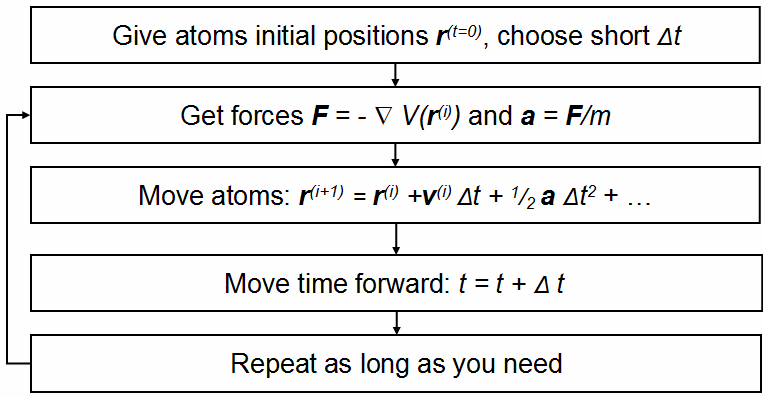
\includegraphics[keepaspectratio, width=0.5\textwidth]{img/md/mdalgorithm.png}
\end{center}
\caption{Esquema general del algoritmo de dinámica molecular}
\label{esquemaMD}
\end{figure}





% *********************
% ****QUE OTROS DATOS RELEVANTES OBTENGO DE LA SIMULACION??
%********************** 

  
El resultado de la simulación es, fundamentalmente, una trayectoria representada por las posiciones de cada una de las partículas a lo largo de un cierto tiempo.
No se va a detallar acerca del análisis posterior de este resultado pero es relevante decir que la longitud de trayectoria que podamos obtener en un tiempo de cómputo razonable es lo que limita el tipo de proceso químico que podremos estudiar.
Para poder estudiar un proceso de interés, entonces, es necesario que la simulación alcance la escala de tiempo en la cual éste ocurre. 
Un mayor tiempo de simulación equivale a realizar más pasos y por lo tanto más cálculos totales, aumentando así el tiempo de cómputo requerido.

Por su parte, simular sistemas más grandes (con mayor cantidad de partículas) implica un incremento en la cantidad de cálculos por cada paso y por lo tanto un mayor costo computacional. 
Además, la función que describe las propiedades del sistema tiene por naturaleza una mayor cantidad de variables, debido a esto es necesario correr la simulación durante más tiempo para poder llegar 
a un conjunto de conformaciones que sea representativo del ensamble real.




\subsection{La función potencial}


En la utilización del método de dinámica molecular, el potencial(V) que permite derivar las fuerzas entre partículas se obtiene modelando al sistema molecular a través de la mecánica clásica (método conocido como mecánica molecular o MM).
Usando un método de MM, se ignoran los electrones y la naturaleza cuántica de estos. La energía potencial del sistema, entonces, depende exclusivamente de las posiciones de los núcleos atómicos. 
Se modela cada molécula como un conjunto de sitios -que representan los átomos que la componen- y resortes -que representan los enlaces químicos entre estos- junto con un potencial parametrizado \textit{ad hoc}.

Este potencial es una función matemática que depende exclusivamente de las posiciones de los átomos, la cual se ajusta a las interacciones observadas experimentalmente entre los componentes del sistema. 
Este tipo de repesentacion simplificada del sistema permite reducir la complejidad de los cálculos necesarios para la simulación y, por lo tanto, el costo computacional asociado. 
La desventaja de este tipo de modelos es que limita el conjunto de procesos que se pueden estudiar. 
Por ej. no es posible hacer análisis de reacciones quimicas que impliquen ruptura o formación de enlaces ya que estos no son considerados con suficiente detalle. 
Mas allá del método MM, existen otras formas de representar al sistema con mayor detalle y aproximaciones que utilizan esquemas híbridos de representación\cite{senn2009qm} buscando balancear el costo computacional y
el detalle que se obtiene del proceso estudiado.
En los ultimos años, surgieron también modelos de representación menos detallados, conocidos como de grano grueso(coarse-grained)\cite{noid2013perspective}, apuntando principalmente a simular sistemas biológicos, que se caracterizan por poseer una gran cantidad de átomos.

Las interacciones representadas en el método de MM se pueden agrupar en dos tipos:

\begin{description}
 \item [De unión:] Describen las interacciones entre dos átomos unidos entre si directamente o hasta dos enlaces de distancia. 
 Consisten en aquellos términos del potencial cuya energía se ve afectada por los estiramientos de los enlaces, las flexiones de los ángulos entre dos átomos, y la rotación de dos átomos adyacentes sobre un eje (ángulos dihedros). Los estiramientos y las flexiones angulares son modeladas mediante un oscilador armónico, mientras que las rotaciones de los enlaces en el plano son modeladas mediante una función trigonométrica.

\item [De no unión:] describen la interacción entre átomos ubicados a más de 3 enlaces de distancia de la misma molécula, o bien entre átomos de moléculas distintas, y consisten en un término para la
contribución electrostática calculada mediante la Ley de Coulomb, y un término para la contribución de Van Der Waals modelada por un potencial de Lennard-Jones 12-6.


\end{description}



El esquema general de la función potencial suele tomar una forma similar al representado en la figura \ref{potencialAmber} \\
% \includegraphics[]{img/ecPotencialAmber.png}
% \begin{figure}[h]
% \includegraphics[keepaspectratio, width=1.0\textwidth]{img/ecPotencialAmber.png}
% \caption{Ejemplo de potencial de interacción del paquete de software Amber}
% \label{Fig:Amber}
% \end{figure}
% \vspace{2pt}
\begin{figure}[!ht]
% \begin{center}
\includegraphics[keepaspectratio, width=\textwidth]{img/md/ecPotencialAmber.png}
% \end{center}
\caption{Ejemplo de potencial de interacción del paquete de software Amber}
% \caption{Esquema general del algoritmo de dinámica molecular}
\label{potencialAmber}
\end{figure}

En azul se representan los términos matemáticos que modelan las interacciones de unión (1. Término de estiramiento de enlaces; 2. Término de flexión angular; 3. Término de rotación de ángulos diedros), y en rojo
las interacciones de no unión (Potencial de Lennard-Jones 12-6 e interacción Coulómbica).

Los parámetros que se observan en esta función potencial (las constantes $K_b, K_{\theta}$ y $V_n$ , los valores de equilibrio $b_0$, $\theta_0$ y $\delta$ , 
las constantes A y B correspondientes al potencial Lennard-Jones, y las cargas q) deben ser ajustados especialmente para cada molécula individual que se desee incluir en la 
simulación. Estos parámetros se suelen obtener tanto de datos experimentales, como así también de rigurosos cálculos cuánticos, y en ocasiones emplean correcciones empíricas.
Al conjunto o "set" de parámetros derivados para utilizarse de forma conjunta en una simulación se lo conoce como campo de fuerzas.

Esta parametrización del modelo de interacciones representa la principal diferencia entre los distintos paquetes de software para simulaciones de dinámica molecular. 
Las distintas versiones suelen tener uno o mas campos de fuerzas propios para utilizar en las simulaciones. 
Estos campos de fuerzas estan parametrizado específicamente para el tipo de sistema que se intenta simular, logrando que se ajuste lo mejor posible a la realidad.
De esta forma, existen versiones específicas para simular distintos sistemas biologicos (proteínas, ácidos nucleicos), otros que intentan abarcar a sistemas de química orgánica en general, etc.
La eleccion del campo de fuerzas es un aspecto importante de la simulacion de DM ya que éste define como se relacionan distintas partes de una misma molécula, como cada átomo se ve afectado por el entorno y como las condiciones contribuyen a la estructura molecular. 

Para estudiar procesos moleculares de interés mediante la técnica de dinámica molecular, es necesario alcanzar la escala correcta de tiempo en la cual ocurre este procesos y, a la vez, asegurarse que el modelado físico
que se está utilizando sea adecuado, de manera que los resultados obtenidos sean precisos.\cite{piana2014assessing}



\subsubsection{Potencial de Lennard-Jones}

El cálculo de las interacciones de no unión es un paso importante en el algoritmo ya que implica la mayor parte del costo computacional asociado a la simulación. 
Esto se debe a que es necesario calcularlo entre todos los elementos del sistema. 
En particular, es importante el término correspondiente al potencial de Lennard-Jones porque este existe siempre, independientemente de la carga neta en las partículas que interaccionan.

La expresión mas común que representa este potencial es: 
\begingroup
\fontsize{14pt}{5pt}
\begin{equation}\label{lennardEquation} V_{LJ}(r)= 4 \epsilon [ (\sigma/r)^{12} - (\sigma/r)^6] \end{equation}
\endgroup
Esta ecuación está compuesta por dos términos representando fuerzas opuestas:
El primer término ($(\sigma/r)^{12}$) representa fuerzas de repulsión que actúan a corta distancia.
El segundo término ($(\sigma/r)^{6}$) representa fuerzas de atracción que actúan en un rango mayor de distancias.

% \vspace{10pt}
Es usual reagrupar los términos $\sigma$ y  $\epsilon$ usando  
$A=4\epsilon\sigma^{12}  $  y  $B=4\epsilon\sigma^6$ para obtener una forma simplificada de la ecuación:   \begin{equation}  V_{LJ}(r)= [ (A/r^{12}) - (B/r^6)] \end{equation}

% \vspace{20pt}


En la figura \ref{lennardimage} se puede ver el comportamiento físico que describe este modelo de interacción:

% ***BUSCAR UNO QUE ESTE ASI DETALLADO PERO EN CASTELLANO****

% \vspace{14pt}
% \begin{center}
% \end{center}

\begin{figure}[!ht]
\centering
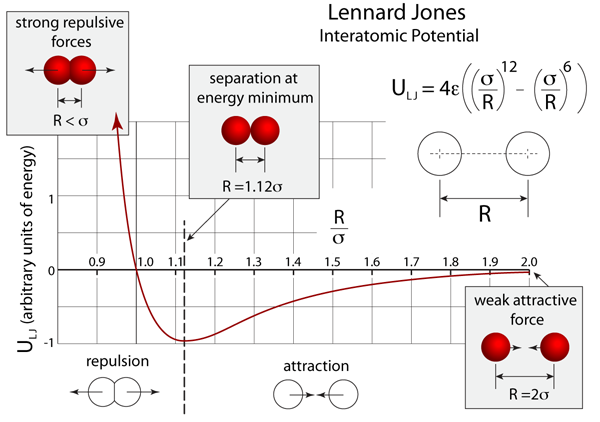
\includegraphics[height=8cm,keepaspectratio, width=\textwidth]{img/md/LennardJonesFull.png}
% \includegraphics[keepaspectratio, height=10cm ,width=0.5\textwidth]{img/minimage.png}
\caption{Comportamiento del potencial de Lennard-Jones}
\label{lennardimage}
\end{figure}

Se pueden observar dos regiones separadas que representan las fuerzas opuestas de la ecuación. 
Estos segmentos están separados por un valor mínimo que se corresponde con el equilibrio entre el componente repulsivo y el de atracción. 
La distancia de equilibrio (que toma un valor de $2^{1/6}\approx1.12$) se obtiene derivando el potencial e igualándolo a 0.

En el primer segmento de la curva ($r<1.12\sigma$), el valor del potencial esta gobernado por el componente repulsivo. 
Este valor aumenta exponencialmente al disminuir la distancia, toma un valor $V=0$ cuando $r=\sigma$, y se hace positivo para valores de $r<\sigma$ indicando una fuerza repulsiva entre los átomos.

En el punto de equilibrio ($r=1.12\sigma$) el potencial toma el valor mínimo $V=-\epsilon$.

En el segundo segmento de la curva ($r>1.12\sigma$), el valor del potencial esta gobernado por el componente atractivo. El valor del potencial (siempre negativo, indicando una fuerza de atracción) se acerca a 0 a medida que la distancia se acerca a infinito. 


A partir de la forma que toma el potencial de L-J resulta razonable pensar que, si se desprecia el aporte de este potencial para interacciones entre partículas a una distancia mayor que cierto valor de corte, 
se podrá obtener una buena aproximación del comportamiento a la vez que se reduce considerablemente la cantidad de cálculos necesarios en cada paso de la simulación.
Esta es una aproximación que proveen varias de las versiones implementadas del método, permitiendo que el usuario defina un valor de corte(\textit{cutoff}). 
En cada paso, si dos partículas están separadas por una distancia mayor que el \textit{cutoff} se les asigna automáticamente un valor de potencial $V_{LJ}=0$ asumiendo que se está realizando una buena aproximación, 
lo que elimina el costo de tener que calcular el valor real. 
Depende del usuario definir un \textit{cutoff} que sea coherente con el sistema y simulación a realizar.

Como se mencionó previamente, el potencial de L-J ofrece una aproximación generalmente buena de las interacciones de no unión en modelos moleculares y, dada su simplicidad, es incluido en gran parte de los campos de fuerzas utilizados en dinámica molecular.
Es por esto que la optimización del calculo asociado tendría un gran impacto en este métdodo de simulación. 
Además, la forma funcional implica que existe, al menos débilmente, entre todos los pares de particulas del sistema, lo que se traduce en una gran cantidad de cálculos por paso. 
El cálculo de este potencial representa así la mayor parte del costo computacional asociado a la simulación. 


\subsection{Condiciones de frontera} \label{frontera}

Hasta aquí hemos definido al sistema como el conjunto de átomos sobre los cuales realizamos la simulación. 
Sin embargo, los sistemas reales tienen, en términos prácticos, un tamaño infinito. 
Es decir, independientemente de cuántos elementos podamos incluir en nuestro conjunto de simulación, el número de parículas(N) será siempre despreciable con respecto al número de componentes del sistema macroscópico real.

Si no se implementa ninguna condición particular a los límites de nuestro sistema, se estaría simulando un conjunto de partículas en el vacío. 
De esta forma, las interacciones ocurrirían solo entre las particulas del conjunto de simulación que definimos, sin tener en cuenta ningún elemento en el contexto.
Además, no habría limites definidos para las posibles posiciones de las partículas, las cuales pueden, por lo tanto, difundir libremente durante la ejecución.

Este tipo de simulaciones raramente es útil ya que no representan situaciones realistas. Se debe tener en cuenta, entonces, condiciones especiales que tendrán los limites en la simulación para que estos representen de forma adecuada a los sistemas de interés.
Existen distintas aproximaciones para implementar estas condiciones en los límites manteniendo un conjunto reducido de partículas.

Utilizar condiciones periódicas de borde es la forma mas común de simular un sistema infinito. Aplicando esta condición, las partículas están contenidas en una caja de simulación con un tamaño definido. 
Esta caja es replicada virtualmente al infinito en las tres direcciones del eje cartesiano, llenando completamente el espacio.
Todas las imágenes de las partículas se mueven de forma idéntica a la partícula central. De hecho, sólo una de ellas(la que se encuentra en la caja central) es la que efectivamente se está simulando.
Cuando una partícula entra o sale de la caja central, una imagen de ella entra o sale por la cara opuesta de esta región, de manera tal que el número de partículas contenidas en la región de simulación siempre se conserva.
Se puede ver que, de esta forma, los límites del sistema que se está simulando son virtualmente eliminados y no tienen ningún efecto sobre la simulación.
Como resultado de esto, cada partícula perteneciente al conjunto de simulación interactúa no solo con las demás partículas de este, sino también con las imágenes virtuales que estamos teniendo en cuenta.

Al parecer, el número de interacciones (y por lo tanto la cantidad de cálculos a realizar) se incrementará enormemente con esta nueva condición. 
Sin embargo, esto puede evitarse si se utiliza un potencial con un rango finito, dado que en este caso se pueden ignorar las interacciones entre partículas separadas por una distancia mayor a cierto valor de \textit{cutoff}.
En este caso, teniendo un valor de cutoff $R_{c}$ y definiendo una caja de simulación cuyo lado menor tenga una longitud $L_m$: 
Si hacemos cumplir que $L_m>2R_{c}$, entonces se verá que, como máximo, solo una de las imágenes de cada particula quedará dentro del rango del cutoff y por lo tanto deberá ser considerada.
Este método, conocido como el criterio de imagen mínima, permite limitar el número de cálculos necesarios considerando solo la imagen mas cercana e ignorando el resto. 
De esta forma se puede cumplir con las características infinitas del sistema real y las propiedades impuestas por el potencial, logrando una mejor aproximación en la simulación.
La figura \ref{minimage} muestra una representación gráfica de este método. 


\begin{figure}[!ht]
\centering
\includegraphics[keepaspectratio, height=10cm ,width=0.5\textwidth]{img/md/minimage.png}
\caption{Criterio de imagen mínima para condiciones periódicas de frontera. Los círculos sin relleno representan todas las imágenes de la misma particula i}
\label{minimage}
\end{figure}


% propiedades fisicas van a depender del tamano de la caja
% Agregar detalles de sumatoria de Ewald ?










\subsection{Estado del arte}



Desde que fue desarrollado, el método ha sido de una gran utilidad y ha demostrado una posiblidad de aplicación a futuro mucho mayor. 
Esta posiblidad de aplicarlo a sistemas cada vez mas grandes y procesos en escalas de tiempo mayores es lo que impulsó una constante búsqueda de mejoras sobre el algoritmo inicial.
Se han desarrollado entonces una gran cantidad de estrategias que apuntan a optimizar el costo computacional asociado al método, sin sufrir una pérdida considerable en la precisión.

Para sistemas típicos de biomoleculas en donde el sistema está compuesto por una macromolécula(ej. proteínas) rodeada de un solvente líquido, es posible utilizar una aproximación conocida 
como solvente implícito\cite{tsui2000theory}.
En este modelo, el solvente se representa como un medio continuo alrededor del sistema central en lugar de representar explícitamente todas las unidades que lo componen, 
reduciendo considerablemente el número de cálculos necesarios para evaluar la interacción con las moléculas de solvente. Al ser una aproximación, tiene ciertas limitaciones en cuanto 
a la precisión y al tipo de sistemas en los que puede ser aplicado.

El calculo asociado al componente electroestático puede ser optimizado usando el método conocido como sumatoria Ewald \cite{toukmaji1996ewald}. 
Este método permite aproximar el cálculo de interacciones que actúan en un amplio rango de distancias sobre sistemas periódicos. 

Otra adaptación muy utilizada es la implementación de una lista de vecinos para cada partícula \cite{plimpton1995fast}. 
Esta lista mantiene las moleculas que estan dentro del rango de interacción(distancia menor al \textit{cutoff}) y son los únicos que se tendrán en cuenta a la hora de hacer el cálculo. 
La optimización se basa en que la lista solo se actualiza cuando se ejecuta una cierta cantidad de pasos definida como parámetro. 
Este valor se deriva experimentalmente a partir de simulaciones de prueba y es el parámetro que balancea la optimización y la precisión: cuanto mas se demora la actualizacién mejor es el 
tiempo de ejecución pero menos representativa es la lista acerca de la realidad del entorno y, por lo tanto, menos preciso es el cálculo.

Existe una gran cantidad de variantes del algoritmo, solo se han mencionado algunos de los caminos en los que se ha avanzado realizando modificaciones con respecto a la descripción inicial.

En cuanto a las arquitecturas de cómputo, las implementaciones sobre GPU, que son el centro de este trabajo, se han establecido como estándares para las implementaciones actuales del método \cite{stone2010gpu,friedrichs2009accelerating}.
Esto se debe al gran poder de cómputo que proveen en relación al costo económico, teniendo en cuenta que el algoritmo es altamente paralelizable y este tipo de hardware provee las condiciones
necesarias para una implementación eficiente.

% 
% Con este contexto , las capacidades de cálculo actuales permiten realizar simulaciones de dinámica molecular en sistemas de hasta XXX átomos aproximadamente, sobre un intervalo de tiempo del 
% orden de YYYYYYY  micro/pico/******segundos).

Si bien se ha avanzado mucho desde el desarrollo del método, existen múltiples procesos de interés que podrían ser abordados mediante experimentos de simulación computacional pero que el intervalo de 
tiempo en el cual ocurren no es posible de ser alcanzado con los recursos disponibles hoy en dia.
Esta situación hace que se destine una gran cantidad de esfuerzo para continuar las mejoras en el método y mantener las implementaciones a la par de las arquitecturas disponibles, 
las cuales han avanzado considerablemente teniendo en cuenta que hace un largo tiempo que el método comenzó a ser aplicado al estudio de proteinas \cite{mccamm0n1977dynamics}
El presente trabajo intenta, entonces, evaluar posibles modificaciones que permitan adecuar las implementaciones más actuales del método para explotar al máximo todas las características 
que ofrece la arquitectura de GPU. 

% ACA PODRIA PONER QUE LOS QUIMICOS TIENEN MUCHOS PROBLEMAS PARA PROBAR LAS COSAS Y BLA BLA BLA YA QUE TIENEN ADAPTACIONES MUY PUNTUALES DEL SISTEMA QUE EJECUTAN ) 
% ADEMAS TENDRIA QUE EXPLICAR EN ALGUN LADO QUE ESTA IMPLEMENTACION SE ENMARCA EN UN PROYECTO  DE MAYOR ESCALA QUE BUSCA IMPLEMENTAR UN ALGORITMO  COARSE-GRAINED
% DESDE CERO, Y  LOS ALGORITMOS COARSE GRAINED SE BASAN EN PROBAR POTENCIALES AD-HOC, A DIFERENCIA DE LOS METODOS MAS DE QM(QUE BUSCAN IR A UNA MENOR ESCALA)
% ENTONCES ES NECESARIO TENER UNA IMPLEMENTACION QUE PERMITA FACILMENTE MODIFICAR LA IMPLEMENTACION

% TAMBIEN PUEDO DECIR QUE UNA IDEA ES TRATAR DE ABSTRAER UN POCO EL PROBLEMA SUBYACENTE Y PLANTEAR LOS COMPONENTES DEL ALGORITMO Y LA FORMA EN QUE ESTOS PUEDEN EVOLUCIONAR HACIA MEJORES PERFORMANCES(YA QUE ).  


